\chapter{Project Focus}
This report is centered about Parental Control (PC) in Smart Home (SH). This chapter will explain what PC and SH is, as well as explorer a field of different possibilities and narrow the possibilities down to a reasonable amount of goals for this project.

%What is smart home
\section{Smart Home}
A Smart Home can refer to multiple forms of improvement on a home. Most commonly is home automation, environment friendly improvements and power saving improvements. In this report we will only regard Smart Home in relation to home automation, however environment friendly- and power saving improvements, sometimes also springs out of home automation. For example if you automate the washing machine to start at a certain hour of the day, it will both be convenient as well as power saving.\\
\\
But a Smart Home, can be much more. Different examples of implementable features is as follows:

\begin{itemize}
	\item Automated security
	\item Music systems
	\item Theater systems
	\item Voice commands
	\item Automatic ordering of groceries
	\item Delayed start on an oven
	\item Automated coffee machines
	\item Light control
	\item Power control on leaving home
	\item And much more
\end{itemize}

This report is about a less common feature of a Smart Home. It is about Parental Control, a concept explained in \ref{parentalControl}.

%What is parental control
\section{Parental Control}
\label{parentalControl}
Parental Control (PC) is a concept most people know from their TV at home or computers. A concept used mainly by parents to protect their children from fx. internet sites with adult content or TV channels of the same kind.\\
But in a Smart Home, this concept could be taken even further. Many electronic devises does not implement a PC feature, and some of those which does, does not allow to block all content.\\
We want to create a system that could help parents manage their children's time. We want to do this in order to improve the well being of children. Studies show that children of the newer ages are sitting indoors, more and more.\citep{childrenAndNature}\citep{leaveNoChildInside}\\
These studies also tell how staying inside both limits the child’s imagination and is a factor for stress. It has also been linked to an increase in likelihood of these children having ADHD.\\
\\
What this project is aiming at is to create a system that would allow the parents to both, help manage their children's time, as well as encourage them to go outside and play.\\
In order for this to succeed, the implementation must offer this control set, without becoming too much of a bother for both the parents and the children it impacts. We do not want to restrict and limit, but rather organize and encourage. - This effectively means, the system can not impose a too long addition to the start up of the restricted devices and the system must implement a feature for the children to earn more time for the restricted devices. These requirements will be gone into further details at a later point REF...

%Write about the brainstorm we did
\section{Potential of Parental Control}
In order to determine the potential for the Parental Control system, a brainstorm was made, to visualize the ideas and couplings that could be made with an existing Smart Home implementation. For this brainstorm we took the base concept of a Smart Home as introduced by Mi Casa Verde\citep{micasaverde}.


\begin{figure}[htbp]
	\centering
		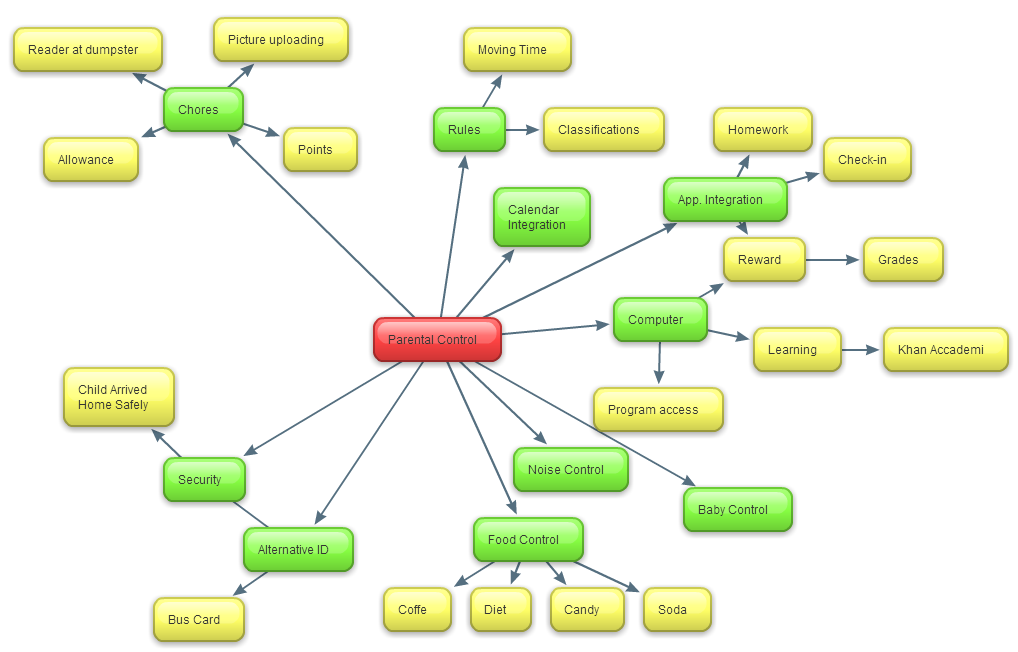
\includegraphics[width=1.00\textwidth]{images/BrainStorm.png}
	\caption{Brainstorm over Parental Control}
	\label{fig:BrainStorm}
\end{figure}

%Explain each point of the Brainstorm, atleast the Green ones, also explain the color codes.
In figure \ref{fig:BrainStorm} is seen 3 different colors. Red is our starting point. Green is our direct sub-points and yellow is our indirect sub-points.\\
Next is a walkthrough of each of the direct sub-points.\\
\subsection{Chores}
\subsection{Rules}
\subsection{Calendar Integration}
\subsection{App. Integration}
\subsection{Computer}
\subsection{Noise Control}
\subsection{Baby Control}
\subsection{Food Control}
\subsection{Alternative ID and Security}


%Narrow down the area we want to covor
%Specify what must be done, in order for it to succed